\documentclass[12pt]{report}
\usepackage[utf8]{inputenc}
\usepackage[T1]{fontenc}
\usepackage{graphicx}
\usepackage[margin=2cm]{geometry}
\usepackage{fancyhdr}
\usepackage{lipsum}


\pagestyle{fancy}
\setlength\headheight{65pt}
\lhead{
\includegraphics[scale=0.4]{logo_phelma.jpg}}
\chead{\large\textbf{Troubleshooting documentation\\ROBOTRONIK PHELMA}}
\rhead{
\includegraphics[scale=0.35]{logoclub.jpg}}
\lfoot{}
\cfoot{\thepage}
\rfoot{}
\renewcommand{\headrulewidth}{0.5pt}
\renewcommand{\footrulewidth}{0.5pt}

\fancypagestyle{plain}{
\setlength\headheight{65pt}
\lhead{
\includegraphics[scale=0.4]{logo_phelma.jpg}}
\chead{\large\textbf{Troubleshooting documentation\\ROBOTRONIK PHELMA}}
\rhead{
\includegraphics[scale=0.35]{logoclub.jpg}}
\lfoot{}
\cfoot{\thepage}
\rfoot{}
\renewcommand{\headrulewidth}{0.5pt}
\renewcommand{\footrulewidth}{0.5pt}
}


\begin{document}
\begin{center}
\Large\textbf{Troubleshooting documentation ROBOTRONIK PHELMA}\normalsize\\
\end{center}
\vspace*{0.5cm}
Finally there are more problems than mentionned in the mail. They will be precised in the following document.


\section*{The Boards :}
\subsection*{The middle control board (the one that control the servomotor) :}
\begin{itemize}
	\item Loose connections between the different boards.
	\item The switches are not functional on two boards (no control over On/Off state).
	\item One board suffers of a power supply problem, which means the power supply is connected but there is no feedback on the board (e.g. LED).
\end{itemize}

\subsection*{Bottom card (the one for the motors and the power electronic) :}
\begin{itemize}
	\item The battery cable is either damaged or missing.
	\item The connectors for the motors were missing in one kit.
	\item As already mentioned, the switches are dysfunctional on two kits.
\end{itemize}

\subsection*{FRDM-KL25Z :}
\begin{itemize}
	\item One of these boards does not work because of an unknown issue, neither connection to the power supply nor to a computer does work.
	\item There are small tin projection, as illustrated in the picture bellow. 
	\begin{center}
		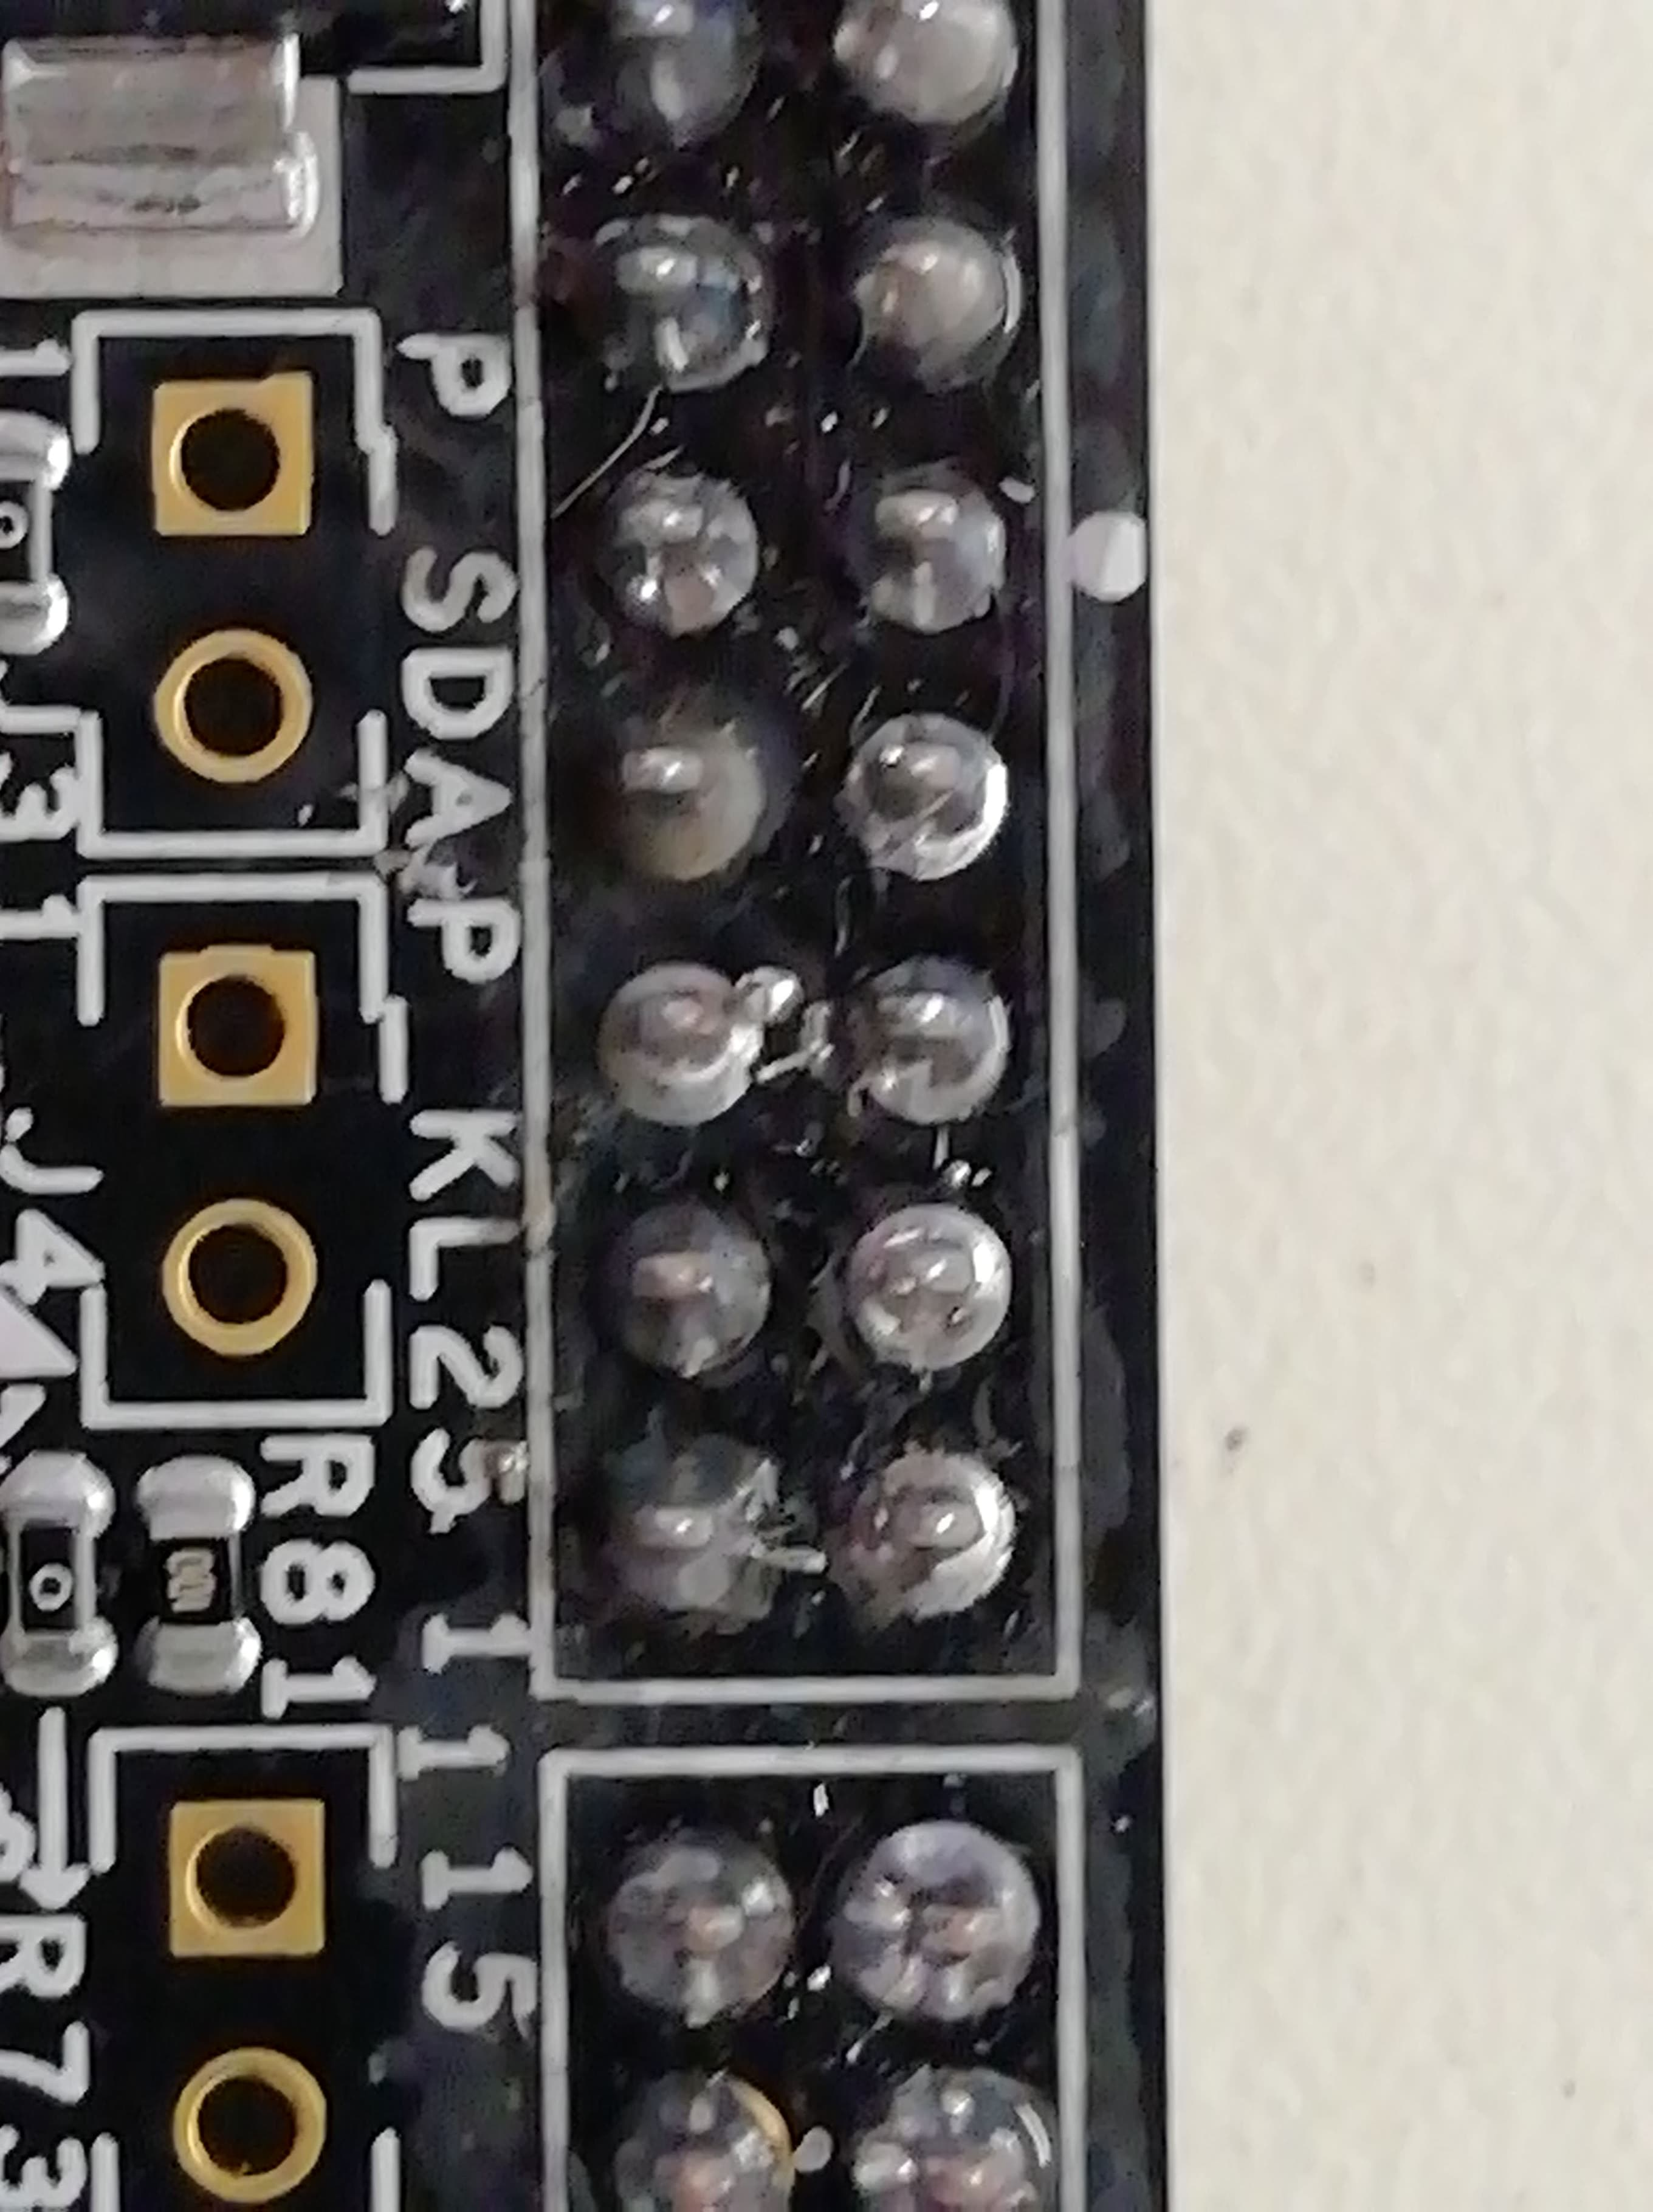
\includegraphics[width=0.35\textwidth]{tinballs.jpg}
	\end{center}
	\item The female jumper casing is damaged on the corners (picture bellow).
	\begin{center}
		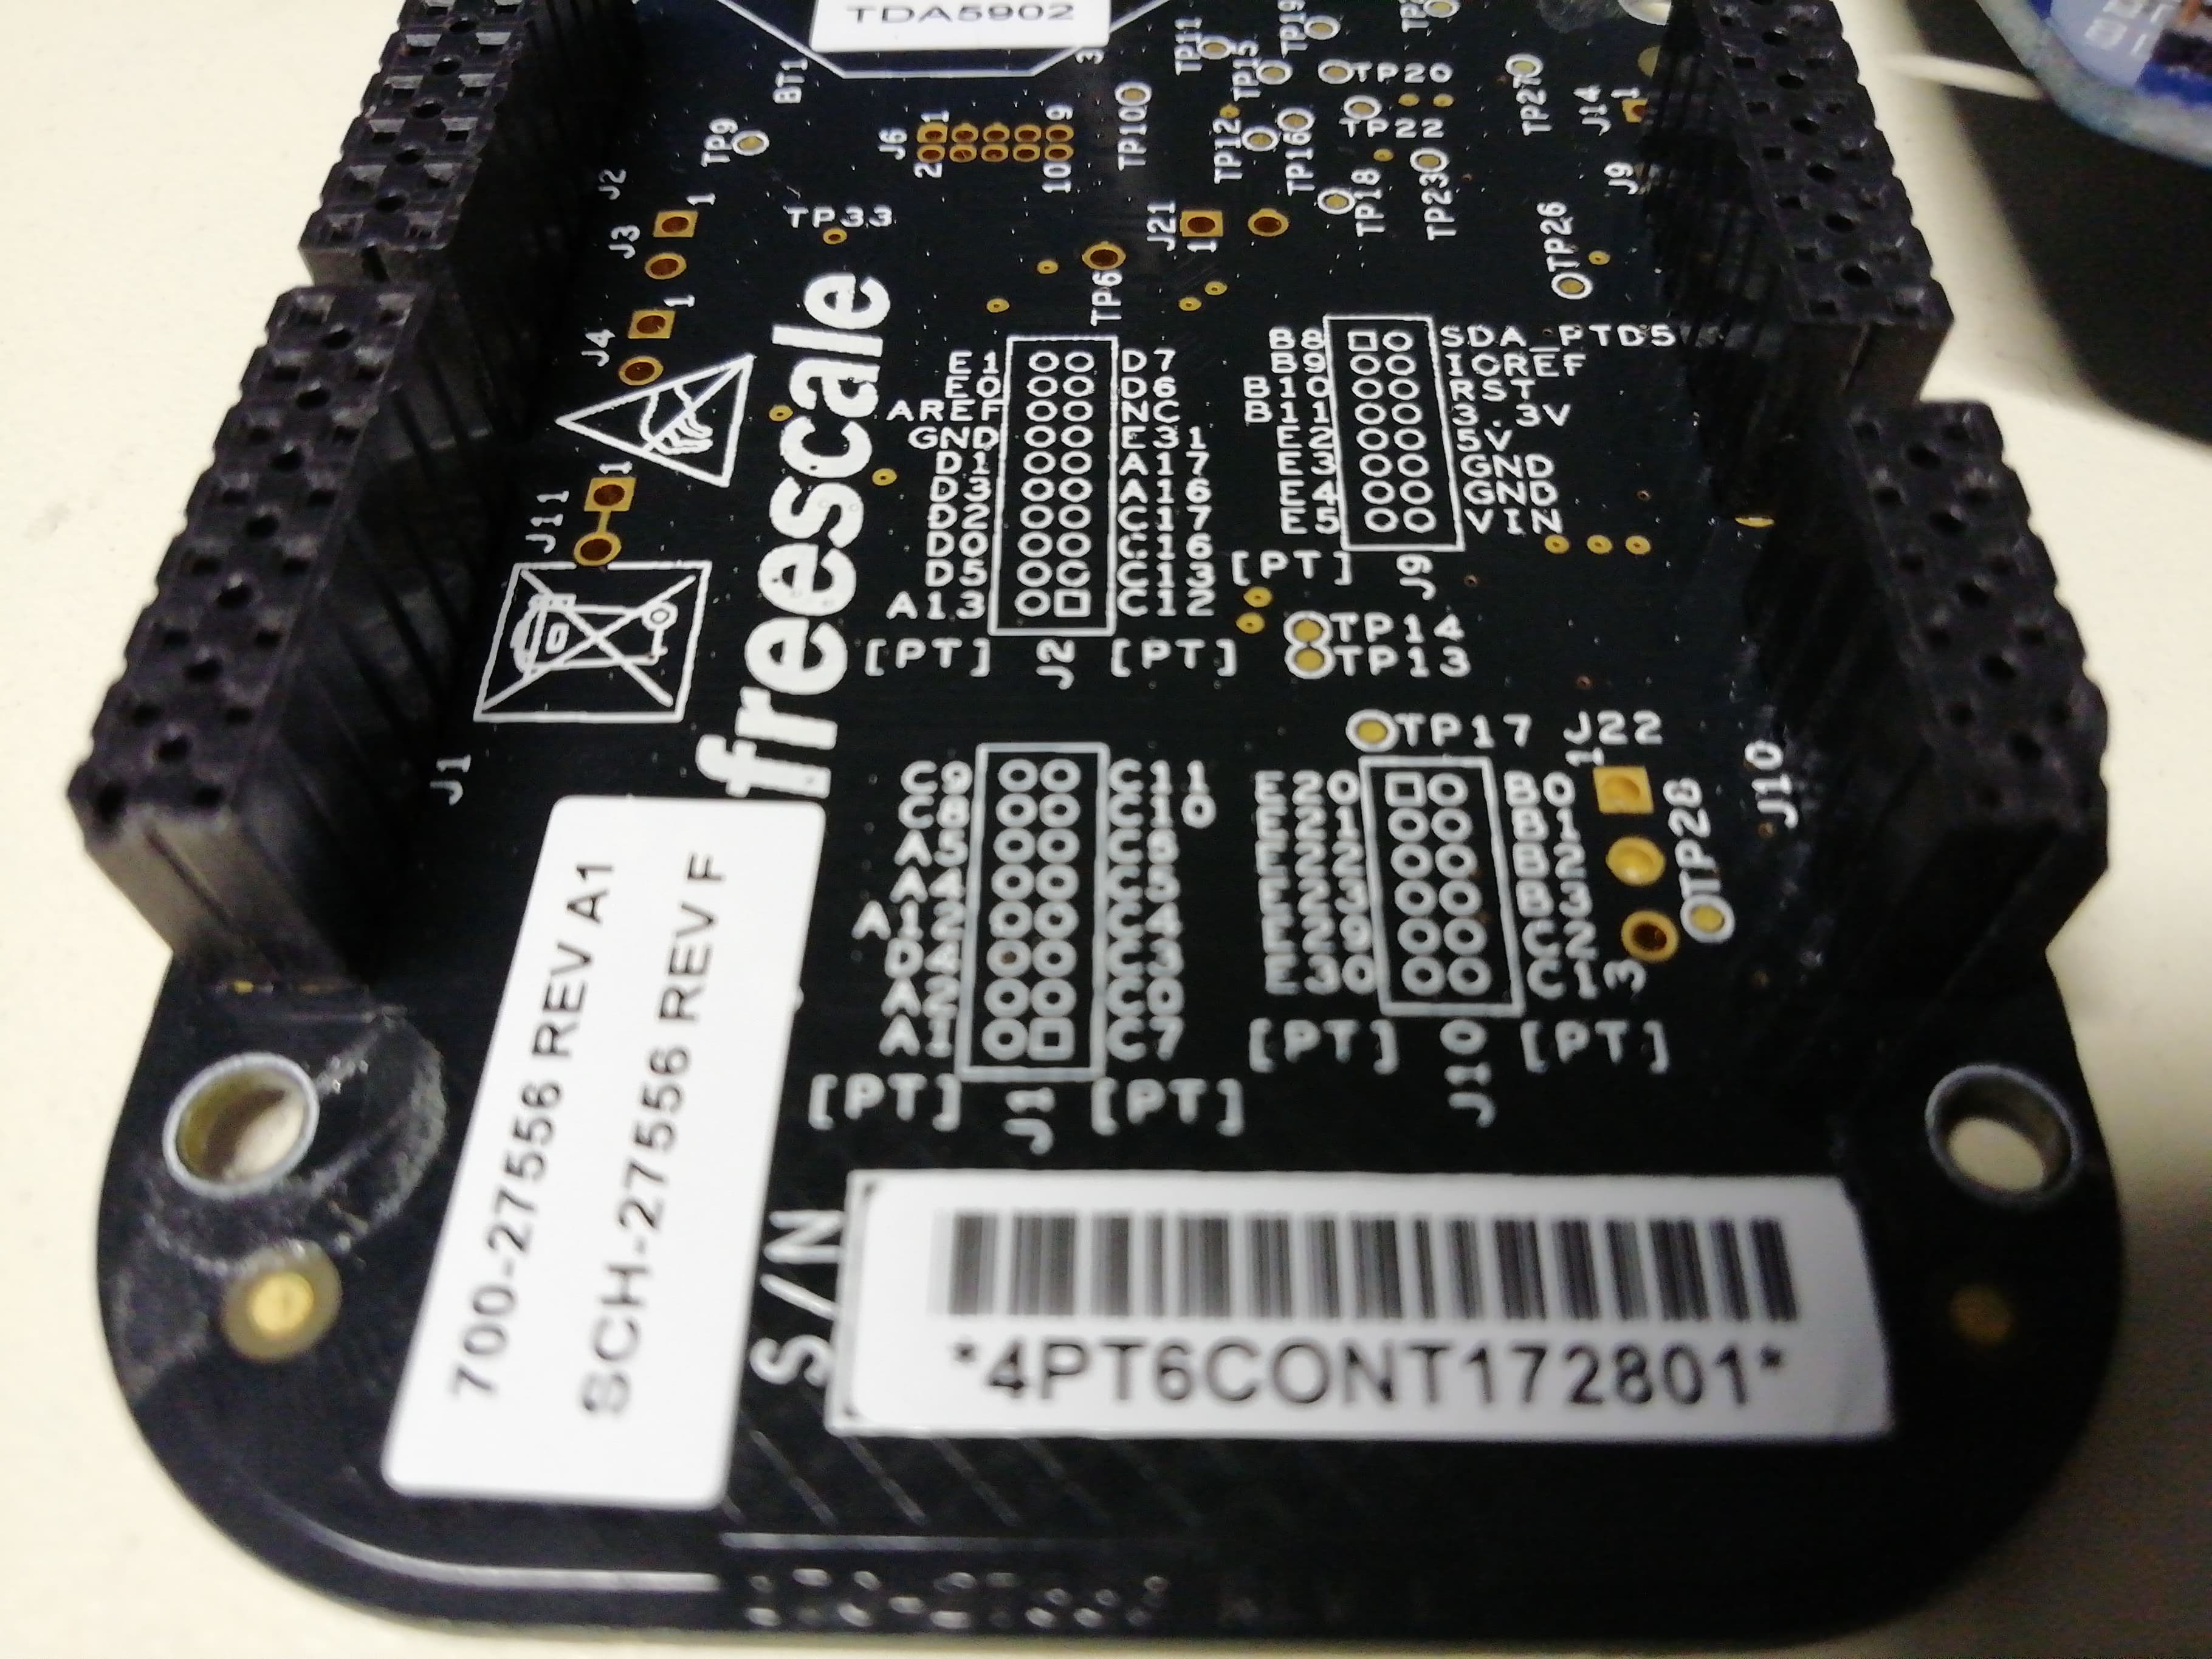
\includegraphics[width=0.35\textwidth]{corner.jpg}
	\end{center}
\end{itemize}


\section*{Camera :}
\begin{itemize}
	\item Connection strip damaged in one kit.
	\item A diode is missing on one camera and causes an inability to use it (cf. picture bellow).
	\begin{center}
		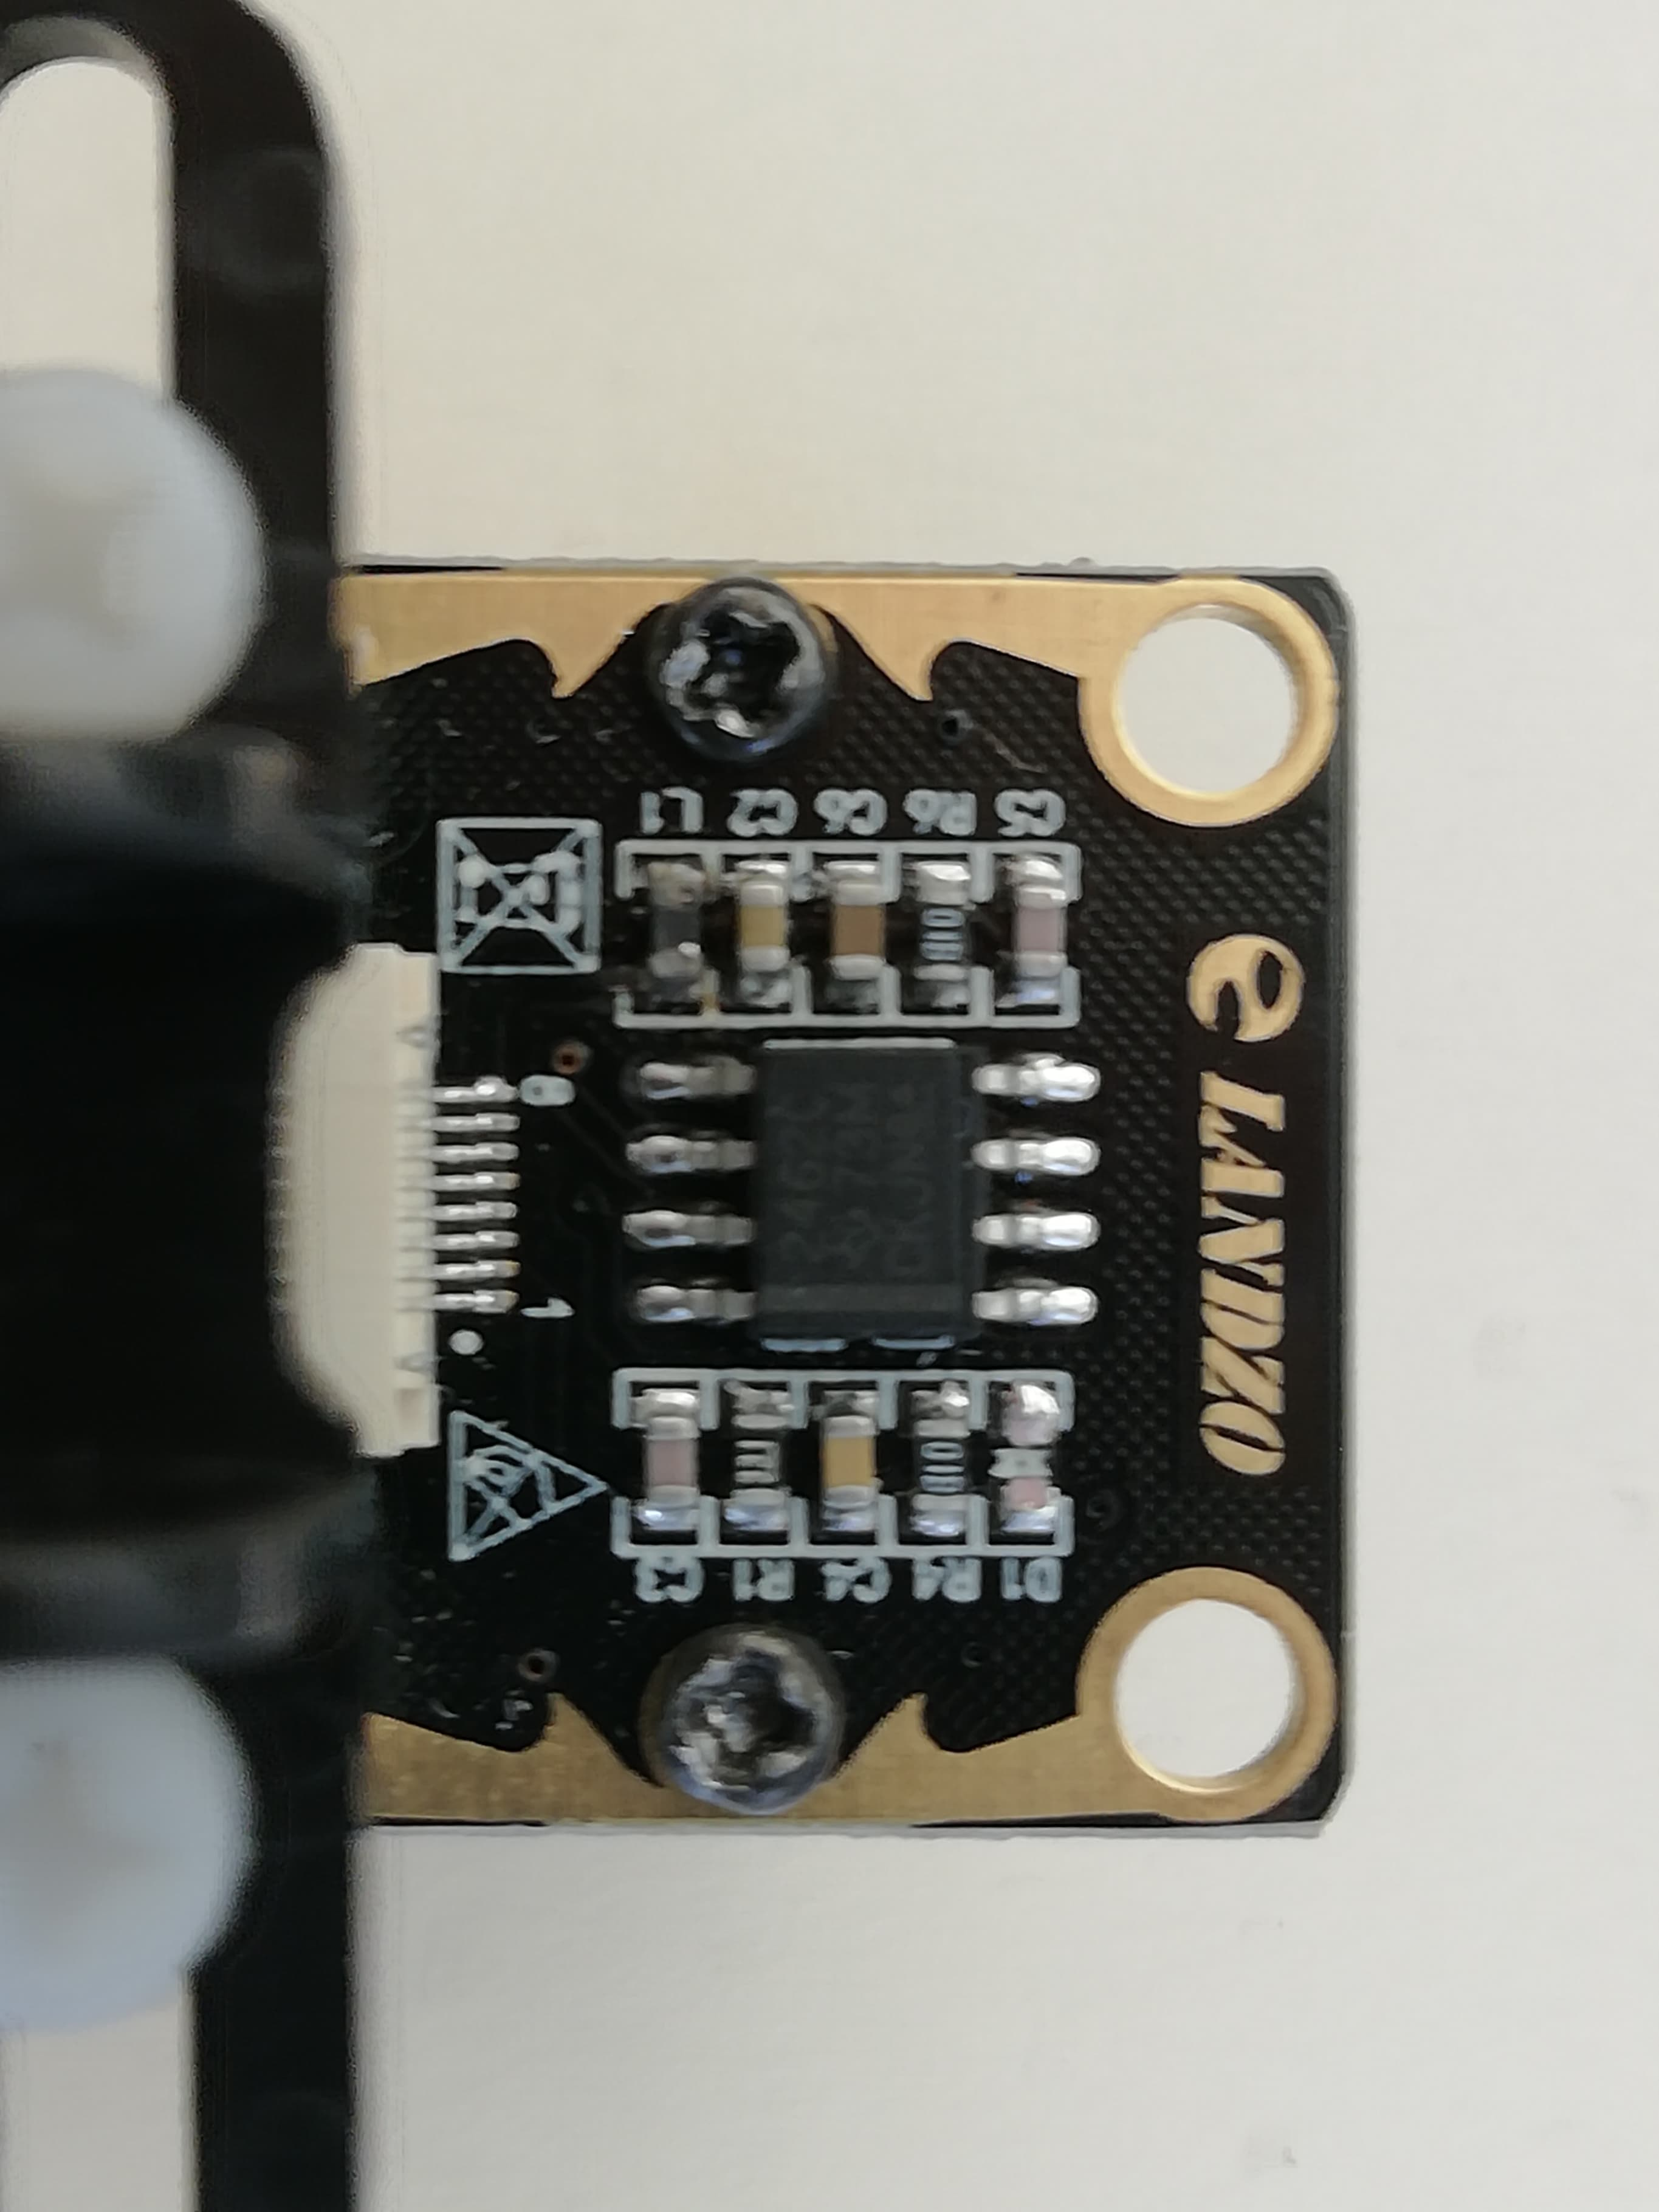
\includegraphics[width=0.35\textwidth]{camera.jpg}
	\end{center}
\end{itemize}

\newpage

\section*{Motors \& Servomotors :}
\subsection*{Motors :}
\begin{itemize}
	\item One motor is out of alignment.
	\item The connectors were not included in any kit.
\end{itemize}
\subsection*{Servomotors :}
\begin{itemize}
	\item The connectors are not adapted to the middle board, which means the cables from the middle board touch the upper board and risk to be broken.
\end{itemize}

\section*{Frame :}
\begin{itemize}
	\item The ankle on the front left wheel is damaged (cf. photo bellow).
	\begin{center}
		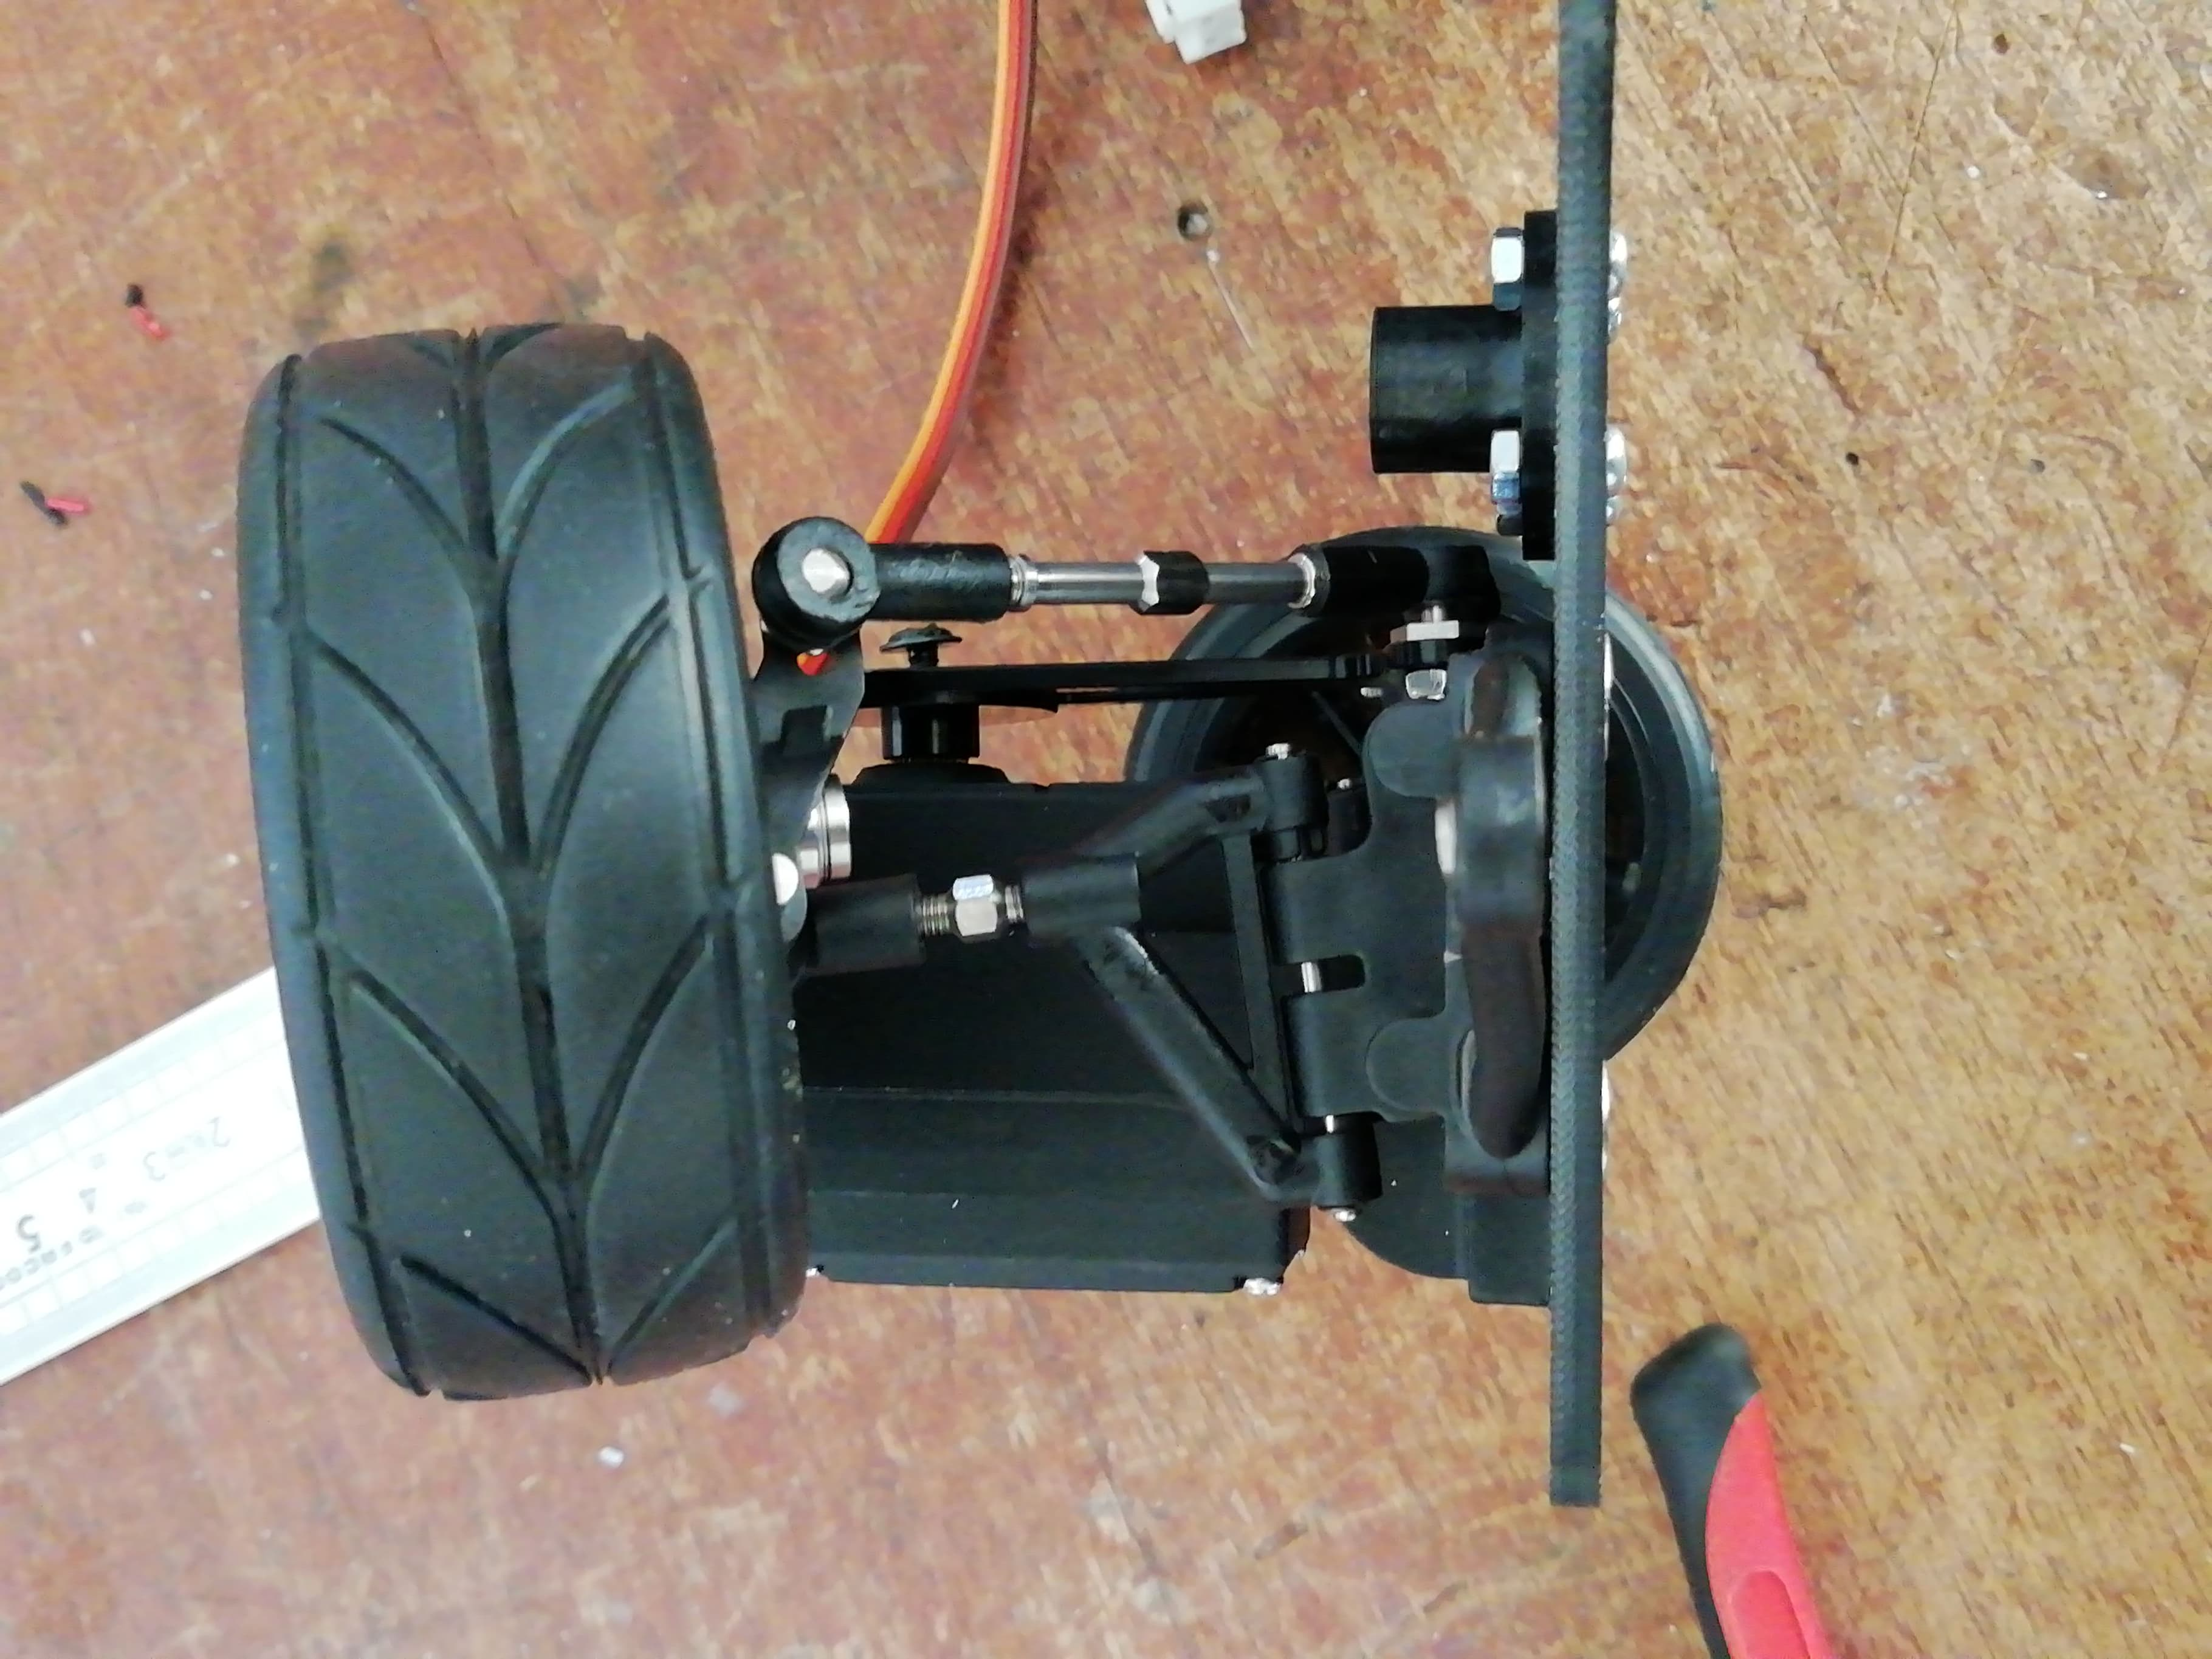
\includegraphics[width=0.4\textwidth]{wheel.jpg}
	\end{center}
\end{itemize}

\newpage

Dear NXP team,

A few days ago, our intern responsable for the NXP Cup received an email to remind the payment of our kits (reference).
In a previous mail sent the .., without any answer, we indicated the first problem we encountered with the kits.
Some problems are still unsolved, news are found and some required extra hardware.
For these reasons we would not be able to participate with our three teams. You will find attached a documentation of all the troubleshooting. 
Is it possible to supply us with change parts ?

Best regards,
Club Robotronik

\end{document}

